\documentclass[border=4pt]{standalone}
\usepackage{tikz}
\usetikzlibrary{shapes.symbols,positioning,arrows.meta}

\begin{document}
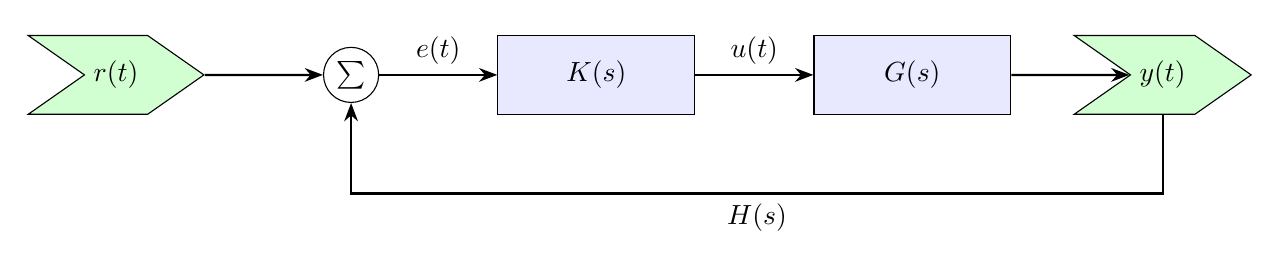
\begin{tikzpicture}[
  >=Stealth,
  node distance=15mm,
  io/.style={signal,signal from=west,signal to=east,signal pointer angle=70,
    draw,minimum width=22mm,minimum height=10mm,fill=green!18},
  block/.style={draw,minimum width=25mm,minimum height=10mm,fill=blue!9},
  flow/.style={->,thick}
]
  \node[io] (reference) {$r(t)$};
  \node[draw,circle,right=of reference,minimum size=7mm,inner sep=0pt] (sum) {$\sum$};
  \node[block,right=of sum] (controller) {$K(s)$};
  \node[block,right=of controller] (plant) {$G(s)$};
  \node[io,right=of plant] (response) {$y(t)$};

  \draw[flow] (reference) -- (sum);
  \draw[flow] (sum) -- node[above]{$e(t)$} (controller);
  \draw[flow] (controller) -- node[above]{$u(t)$} (plant);
  \draw[flow] (plant) -- (response);
  \draw[flow] (response.south) -- ++(0,-10mm) -| node[pos=.25,below]{$H(s)$} (sum.south);
\end{tikzpicture}
\end{document}
